\begin{subfigure}[b]{0.31\textwidth}
        \centering
        \begin{tikzpicture}
        \foreach \line [count=\y] in \pixelsOneZero {
    			\foreach \pix [count=\x] in \line {
      			\draw[fill=pixel \pix] (\x/\scaleSmall,-\y/\scaleSmall) rectangle +(1/								\scaleSmall,1/\scaleSmall);
    			}
  		}
        \end{tikzpicture}
        \caption{$10\times10$}  
        \label{fig:10x10}
    \end{subfigure}
    \quad
    \begin{subfigure}[b]{0.31\textwidth}  
        \centering 
        \begin{tikzpicture}
	    \foreach \line [count=\y] in \pixelsOneSeven {
    			\foreach \pix [count=\x] in \line {
      			\draw[fill=pixel \pix] (\x/\scaleMiddle,-\y/\scaleMiddle) rectangle +(1/								\scaleMiddle,1/\scaleMiddle);
    			}
  		}
        \end{tikzpicture}
        \caption{$17\times17$}   
        \label{fig:17x17}
    \end{subfigure}
    \quad
    \begin{subfigure}[b]{0.31\textwidth}   
        \centering 
        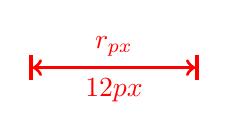
\begin{tikzpicture}
  		\foreach \line [count=\y] in \pixelsTwoFour {
    			\foreach \pix [count=\x] in \line {
      			\draw[fill=pixel \pix] (\x/\scaleBig,-\y/\scaleBig) rectangle +(1/								\scaleBig,1/\scaleBig);
    			}
  		}
  		\draw[very thick,|<->|,red] (2.55,-2.4) -- (4.7,-2.4) node[midway, below, fill=white]{$\SI{12}{px}$} node[midway, above, fill=white]{$r_{\text{px}}$};
        \end{tikzpicture}
        \caption{$25\times25$}    
        \label{fig:25x25}
    \end{subfigure}